




\section{Benchmarking \& Results}
\label{sec:benchmarking}

In this section, we benchmark \coolname across a wide suite of 3D vision tasks.
For each task, we compare against expert baselines specifically designed or trained for the task.
We perform all experiments with a constant seed.



\paragraph{Multi-View Dense Reconstruction:}

We benchmark the performance of pointmaps, pose, depth \& ray direction estimation on an undistorted version of ETH3D \cite{SchoepSGSSPG2017}, ScanNet++ v2 \cite{YeshwLND2023}, and TartanAirV2-WB \cite{WangZWHQWHKS2020, ZhangKLJCQKJHRSW2025}, where, for each test scene, we randomly sample up to $N$ views that form a single connected component graph based on the pre-computed pairwise covisibility of all images in the scene (this prevents disjoint sets of images as input).
\cref{fig:comparison_graphs} shows that \coolname provides state-of-the-art dense multi-view reconstruction performance over other baselines using only image input, including VGGT \cite{WangCKVRN2025}.
Beyond the performance using only images as input, we show that \coolname can leverage additional auxiliary geometric inputs for feed-forward inference to further increase reconstruction performance by a significant factor.
Furthermore, we find that \coolname is better than the bundle adjustment (BA) variant of the two-view baseline, Pow3R \cite{JangWLAR2025}, which is also designed to leverage scene priors.
We also find that reconstruction outputs from \coolname (using only images as input) display high fidelity, as shown in \cref{fig:qual_comparison}. 

\begin{figure*}[!t]
    \centering
    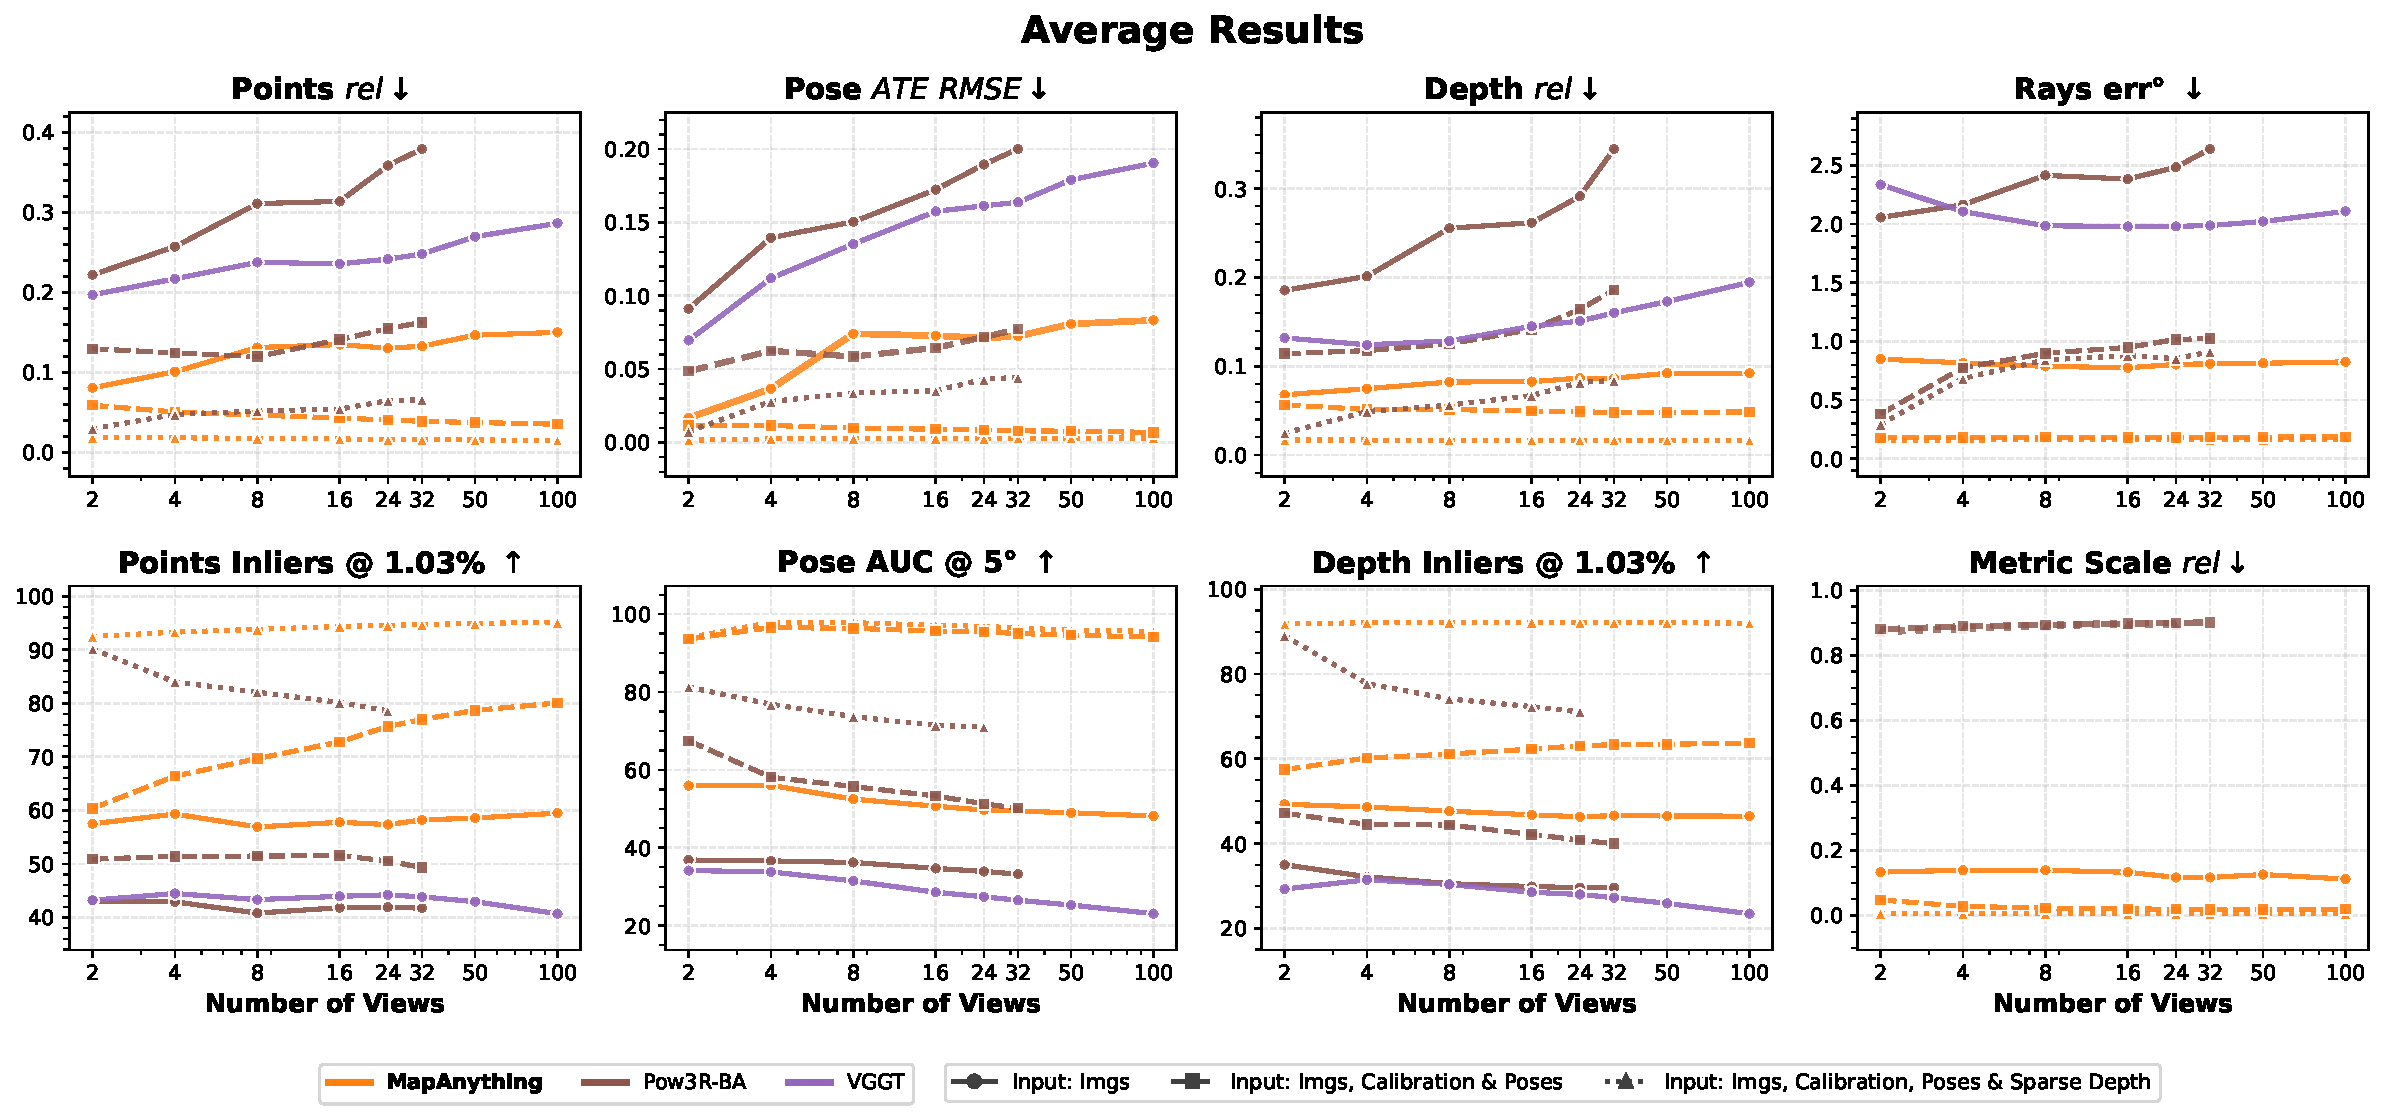
\includegraphics[trim={0cm 0cm 0cm 0.9cm},clip,width=\linewidth]{figs/V1_1_Benchmarking/v1_1_bench/results_v1_1_bench_average.pdf}
    \caption{\label{fig:comparison_graphs}%
    \textbf{\coolname shows state-of-the-art dense multi-view reconstruction for input views ranging from 2 to 100 and under different input configurations.}
    We report the absolute relative error ($\absrel$), the inlier ratio at a relative threshold of $1.03\%$ ($\threshI$), the average aligned trajectory error ($ATE~RMSE$), the area under the curve at an error threshold of 5° ($AUC@5$), and the average angular error ($err$) in degrees (°), averaged over ETH3D, ScanNet++ v2 \& TAv2.
    We do not report performance for baselines when the inference runs out of GPU memory.
    We provide results for individual datasets \& the exhaustive input configurations of \coolname in the supplement.
    }
\end{figure*}


\paragraph{Two-View Dense Reconstruction:}

We benchmark sparse-view reconstruction and image-matching performance against state-of-the-art feed-forward baselines in \cref{tab:two_view_dense_recon}.
\coolname achieves state-of-the-art performance using only images as input.
With additional input modalities, \coolname significantly outperforms both image-only baselines and Pow3R \cite{JangWLAR2025}, the only other two-view feed-forward method that uses scene or camera priors.



\begin{table}[t]
\caption{\label{tab:two_view_dense_recon}%
  \textbf{\coolname showcases state-of-the-art two-view reconstruction under different input configurations.} We report the absolute relative error ($\absrel$), the inlier ratio at a relative threshold of 1.03\% ($\threshI$), the average aligned trajectory error (ATE), the area under the curve at an error threshold of 5° (AUC), and the average angular error ($err$) in degrees (°). Best results are indicated in \textbf{bold}.
}
\centering
\scriptsize
\setlength\tabcolsep{2pt}
\resizebox{\columnwidth}{!}{%
\begin{tabular}{l@{\hspace{8pt}}c@{\hspace{8pt}}c@{\hspace{6pt}}c@{\hspace{8pt}}cc@{\hspace{8pt}}c@{\hspace{6pt}}c@{\hspace{8pt}}c}
\toprule
& \multicolumn{8}{c}{\textbf{Average across ETH3D, SN++v2 \& TAV2}} \\
\cmidrule(lr){2-9}
& \multicolumn{1}{c@{\hspace{8pt}}}{\textbf{Scale}}
& \multicolumn{2}{c@{\hspace{8pt}}}{\textbf{Points}}
& \multicolumn{2}{c@{\hspace{8pt}}}{\textbf{Pose}}
& \multicolumn{2}{c@{\hspace{8pt}}}{\textbf{Depth}}
& \multicolumn{1}{c}{\textbf{Rays}} \\
\textbf{Methods}
& $\absrel\downarrow$
& $\absrel\downarrow$
& $\threshI\uparrow$
& \scriptsize ATE $\downarrow$
& \scriptsize AUC $\uparrow$
& $\absrel\downarrow$
& $\threshI\uparrow$
& err° $\downarrow$ \\
\midrule
\multicolumn{9}{l}{\textbf{a) Input: Images}} \\
DUSt3R~\cite{WangLCCR2024}     & ---   & 0.21    & 43.9    & 0.08   & 35.5    & 0.17   & 32.6    & 2.55    \\
MASt3R~\cite{LeroyCR2024}     & 0.38   & 0.25    & 30.2    & 0.07   & 37.3    & 0.19   & 24.8    & 7.03    \\
Pow3R~\cite{JangWLAR2025}     & ---   & 0.22    & 43.1    & 0.09   & 36.9    & 0.19   & 35.0    & 2.06    \\
VGGT~\cite{WangCKVRN2025}     & ---   & 0.20    & 43.2    & 0.07   & 34.2    & 0.13   & 29.3    & 2.34    \\
\textbf{{\coolname}}     & \textbf{0.13}   & \textbf{0.08}    & \textbf{57.5}    & \textbf{0.02}   & \textbf{56.0}    & \textbf{0.07}   & \textbf{49.3}    & \textbf{0.85}    \\

\arrayrulecolor{gray}\midrule
\multicolumn{9}{l}{\textbf{b) Input: Images \& Intrinsics}} \\
Pow3R~\cite{JangWLAR2025}     & ---   & 0.20    & 46.0    & 0.08   & 51.3    & 0.15   & 43.2    & 0.40    \\
\textbf{{\coolname}}     & \textbf{0.13}   & \textbf{0.07}    & \textbf{59.3}    & \textbf{0.01}   & \textbf{64.7}    & \textbf{0.06}   & \textbf{55.1}    & \textbf{0.19}    \\

\midrule
\multicolumn{9}{l}{\textbf{c) Input: Images, Intrinsics \& Poses}} \\
Pow3R~\cite{JangWLAR2025}     & ---   & 0.13    & 50.9    & 0.05   & 67.5    & 0.11   & 47.2    & 0.38    \\
\textbf{{\coolname}}     & \textbf{0.05}   & \textbf{0.06}    & \textbf{60.4}    & \textbf{0.01}   & \textbf{93.6}    & \textbf{0.06}   & \textbf{57.5}    & \textbf{0.18}    \\

\midrule
\multicolumn{9}{l}{\textbf{d) Input: Images, Intrinsics \& Depth}} \\
Pow3R~\cite{JangWLAR2025}     & ---   & 0.13    & \textbf{77.9}    & 0.04   & 66.5    & 0.07   & \textbf{77.3}    & 0.29    \\
\textbf{{\coolname}}     & \textbf{0.02}   & \textbf{0.04}    & 77.8    & \textbf{0.01}   & \textbf{73.1}    & \textbf{0.03}   & 76.6    & \textbf{0.18}    \\

\midrule
\multicolumn{9}{l}{\textbf{e) Input: Images, Intrinsics, Poses \& Depth}} \\
Pow3R~\cite{JangWLAR2025}     & ---   & 0.03    & \textbf{90.1}    & 0.01   & 81.3    & 0.02   & \textbf{89.0}    & 0.29    \\
\textbf{{\coolname}}     & \textbf{0.01}   & \textbf{0.02}    & 82.0    & \textbf{0.00}   & \textbf{94.8}    & \textbf{0.02}   & 81.5    & \textbf{0.16}    \\

\arrayrulecolor{black}\bottomrule
\end{tabular}%
}
\end{table}















\paragraph{Single-View Calibration:}

We benchmark the single-view calibration performance of \coolname and other expert calibration baselines on randomly sampled frames from the test scenes of undistorted ETH3D \cite{SchoepSGSSPG2017}, ScanNet++ v2 \cite{YeshwLND2023}, and TartanAirV2 \cite{WangZWHQWHKS2020}.
To test non-centered principal points, we randomly crop frames with aspect ratios from 3:1 to 1:2.
Despite not being trained specifically on single images, \cref{tab:single_view_calib} shows that \coolname achieves state-of-the-art performance for perspective calibration.
This demonstrates \coolname's effectiveness in modeling generic central camera systems
and its potential to generalize to wide-angle models like fisheye with appropriate training.

\begin{table}[t]
\caption{\label{tab:single_view_calib}%
    \textbf{\coolname shows state-of-the-art single-image calibration.} Note that \coolname has not been trained specifically for single-image inputs. We report the average angular error ($err$) in degrees (°). Best results are indicated in \textbf{bold}.
}
\centering
\scriptsize
\begin{tabular}{lcccc}
\toprule


    \textbf{Methods}
    & \multicolumn{1}{c}{\textbf{Avg.}}
    & \multicolumn{1}{c}{\textbf{ETH3D}}
    & \multicolumn{1}{c}{\textbf{SN++v2}}
    & \multicolumn{1}{c}{\textbf{TAV2}}
    \\

    \midrule

    VGGT~\cite{WangCKVRN2025}
    & 4.00
    & 2.83
    & 5.21
    & 3.95
    \\

    MoGe-2~\cite{WangXDDXLSTY2025}
    & 1.95
    & 1.89
    & 1.56
    & 2.40
    \\

    AnyCalib~\cite{TiradC2025}
    & 2.01
    & 1.52
    & 2.41
    & 2.10
    \\



    \textbf{\coolname}
    & \textbf{1.06}
    & \textbf{1.33}
    & \textbf{0.39}
    & \textbf{1.47}
    \\

\bottomrule
\end{tabular}
\end{table}



\begin{table}[t]
    \caption{\label{tab:robust-multi-view-depth}%
        \textbf{\coolname shows versatile metric depth estimation under different input configurations on the Robust-MVD Benchmark \cite{SchroeBAB2022}}.
        Note that \coolname has not been trained for single-image inputs.
        We report the absolute relative error ($\absrel$) and the inlier ratio at a relative threshold of 1.03\% ($\threshI$).
        The best result for each group is in \bestresult{bold}; \textcolor{lightgray}{gray text} indicates results where the evaluation dataset is in the training distribution~\cite{IzquiSFGTCABW2025}.
    }
    \scriptsize
    \centering
        \def\pad{\phantom{0}}
\begin{tabular}{l
@{\hspace{6pt}}c
@{\hspace{6pt}}c
c c
c c
}

\toprule
    &
    &
    & \multicolumn{2}{c}{\textbf{KITTI}}
    & \multicolumn{2}{c}{\textbf{ScanNet}}
    \\

    \textbf{Approach}
    & \textbf{K}
    & \textbf{Poses}
    & $\absrel\downarrow$ & $\threshI\uparrow$
    & $\absrel\downarrow$ & $\threshI\uparrow$
    \\

    \midrule

    \multicolumn{7}{l}{\textbf{a) Single-View Metric}}
    \\[0.4em]

        MoGe-2~\cite{WangXDDXLSTY2025}
        & \xmark
        & \xmark
        & 14.21
        & \pad 6.8
        & \pad \textbf{10.57}
        & \textbf{19.8}
        \\



        \textbf{\coolname}
        & \xmark
        & \xmark
        & \pad\textbf{9.69}
        & \textbf{17.9}
        & \pad 27.77
        & \pad 2.9
        \\

    \arrayrulecolor{lightgray}\midrule

        Depth Pro~\cite{BochkDGSZRK2025}
        & \tickmark
        & \xmark
        & 13.60
        & 14.3
        & \pad\pad\textcolor{lightgray}{9.20}
        & \textcolor{lightgray}{19.7}
        \\

        UniDepthV2~\cite{PicciSYSLAV2026}
        & \tickmark
        & \xmark
        & 13.70
        & \pad 4.8
        & \pad\pad\textcolor{lightgray}{3.20}
        & \textcolor{lightgray}{61.3}
        \\

        Metric3DV2~\cite{HuYZCLCWYSS2024}
        & \tickmark
        & \xmark
        & \pad8.70
        & 13.2
        & \pad\pad\textcolor{lightgray}{6.20}
        & \textcolor{lightgray}{19.3}
        \\



        \textbf{\coolname}
        & \tickmark
        & \xmark
        & \pad\textbf{8.48}
        & \textbf{27.7}
        & \pad\textbf{31.12}
        & \pad\textbf{3.0}
        \\

    \arrayrulecolor{gray}\midrule

    \multicolumn{7}{l}{\textbf{b) Multi-View Metric}}
    \\[0.4em]

        MAST3R~\cite{LeroyCR2024}
        & \xmark
        & \xmark
        & 61.40 %
        & \pad 0.4
        & \pad\textcolor{lightgray}{12.80} %
        & \textcolor{lightgray}{19.4}
        \\

        MUSt3R~\cite{CabonSACCRL2025}
        & \xmark
        & \xmark
        & 19.76
        & \pad 7.3
        & \pad\pad\textcolor{lightgray}{7.66}
        & \textcolor{lightgray}{35.7}
        \\ %
    


        \textbf{\coolname}
        & \xmark
        & \xmark
        & \pad\textbf{5.45}
        & \textbf{45.7}
        & \pad\textbf{22.23}
        & \textbf{10.6}
        \\

    \arrayrulecolor{lightgray}\midrule


        \textbf{\coolname}
        & \tickmark
        & \xmark
        & \pad\textbf{8.45}
        & \textbf{27.5}
        & \pad\textbf{24.94}
        & \pad\textbf{8.2}
        \\

    \arrayrulecolor{lightgray}\midrule

        Fast-MVSNet~\cite{YuG2020}
        & \tickmark
        & \tickmark
        & 12.10
        & 37.4
        & 287.10
        & \pad 9.4
        \\ %
    
    
    
        Robust MVDB~\cite{SchroeBAB2022}
        & \tickmark
        & \tickmark
        & \pad 7.10
        & 41.9
        & \pad\pad 7.40
        & 38.4
        \\ %
    
        MAST3R Tri.~\cite{IzquiSFGTCABW2025}
        & \tickmark
        & \tickmark
        & \pad 3.40
        & 66.6
        & \pad\pad\textcolor{lightgray}{4.50}
        & \textcolor{lightgray}{63.0}
        \\ %
    
        MVSA~\cite{IzquiSFGTCABW2025}%
        & \tickmark
        & \tickmark
        & \pad\bestresult{3.20}
        & \bestresult{68.8}
        & \pad \pad\bestresult{3.70}
        & \bestresult{62.9}
        \\
    


        \textbf{\coolname}
        & \tickmark
        & \tickmark
        & \pad 4.63
        & 51.6
        & \pad \pad 5.58
        & 48.1
        \\ %

    \midrule

    \multicolumn{7}{l}{\textbf{c) Single-View w/ Alignment}}
    \\[0.4em]

        MoGe~\cite{WangXDXDTY2025}
        & \xmark
        & \xmark
        & \pad 5.12
        & 46.2 %
        & \pad\pad\textbf{3.59}
        & \textbf{65.3} %
        \\

        MoGe-2~\cite{WangXDDXLSTY2025}
        & \xmark
        & \xmark
        & \pad\textbf{4.82}
        & \textbf{47.9} %
        & \pad\pad3.77
        & 63.1 %
        \\

        VGGT~\cite{WangCKVRN2025}
        & \xmark
        & \xmark
        & \pad7.50
        & 33.0 %
        & \pad\pad\textcolor{lightgray}{3.33}
        & \textcolor{lightgray}{70.8} %
        \\

        $\pi^3$~\cite{WangZZCZLCPSH2025}
        & \xmark
        & \xmark
        & \pad6.00
        & 40.1
        & \pad\pad\textcolor{lightgray}{2.90}
        & \textcolor{lightgray}{73.9}
        \\


        \textbf{\coolname}
        & \xmark
        & \xmark
        & \pad6.12
        & 42.2
        & \pad \pad 4.95
        & 55.6
        \\
        
    \arrayrulecolor{lightgray}\midrule

        Depth Pro~\cite{BochkDGSZRK2025}
        & \tickmark
        & \xmark
        & \pad 6.10
        & 39.6
        & \pad\pad\textcolor{lightgray}{4.30}
        & \textcolor{lightgray}{58.4}
        \\

        DAV2~\cite{YangKHZXFZ2024}
        & \tickmark
        & \xmark
        & \pad 6.60
        & 38.6
        & \pad\pad\textbf{4.00}
        & \textbf{58.6}
        \\ %

        Metric3DV2~\cite{HuYZCLCWYSS2024}
        & \tickmark
        & \xmark
        & \pad 5.10
        & 44.1
        & \pad\pad\textcolor{lightgray}{2.40}
        &  \textcolor{lightgray}{78.3}
        \\

        UniDepthV2~\cite{PicciSYSLAV2026}
        & \tickmark
        & \xmark
        & \pad\bestresult{4.00}
        & \bestresult{55.3}
        & \pad\pad\textcolor{lightgray}{2.10}
        & \textcolor{lightgray}{82.6}
        \\


        \textbf{\coolname}
        & \tickmark
        & \xmark
        & \pad6.15
        & 41.6
        & \pad\pad 4.77
        & 57.1
        \\

    \midrule

    \multicolumn{7}{l}{\textbf{d) Multi-View w/ Alignment}}
    \\[0.4em]

        MAST3R~\cite{LeroyCR2024}
        & \xmark
        & \xmark
        & \pad3.30
        & 67.7
        & \pad\pad\textcolor{lightgray}{4.30}
        & \textcolor{lightgray}{64.0}
        \\ %

        MUSt3R~\cite{CabonSACCRL2025}
        & \xmark
        & \xmark
        & \pad 4.47
        & 56.7
        & \pad\pad\textcolor{lightgray}{3.22}
        & \textcolor{lightgray}{69.2}
        \\ %

        VGGT~\cite{WangCKVRN2025}
        & \xmark
        & \xmark
        & \pad 4.60
        & 53.0 %
        & \pad\pad\textcolor{lightgray}{2.34}
        & \textcolor{lightgray}{80.6} %
        \\

        $\pi^3$~\cite{WangZZCZLCPSH2025}
        & \xmark
        & \xmark
        & \pad\textbf{3.09}
        & \textbf{69.5}
        & \pad\pad\textcolor{lightgray}{1.98}
        & \textcolor{lightgray}{83.6}
        \\


        \textbf{\coolname}
        & \xmark
        & \xmark
        & \pad 4.04
        & 60.3
        & \pad\pad\textbf{3.47}
        & \textbf{67.0}
        \\

    \arrayrulecolor{lightgray}\midrule

        DeMoN~\cite{UmmenZUMIDB2017}
        & \tickmark
        & \xmark
        & 15.50
        & 15.2
        & \pad 12.00
        & 21.0
        \\ %
    
        DeepV2D {\scriptsize{KITTI}}~\cite{TeedD2020}
        & \tickmark
        & \xmark
        & \pad\textcolor{lightgray}{3.10}
        & \textcolor{lightgray}{74.9}
        & \pad 23.70
        & 11.1
        \\ %
    
        DeepV2D {\scriptsize{ScanNet}}~\cite{TeedD2020}
        & \tickmark
        & \xmark
        & 10.00
        & 36.2
        & \pad\pad\textcolor{lightgray}{4.40}
        & \textcolor{lightgray}{54.8}
        \\ %
    

        \textbf{\coolname}
        & \tickmark
        & \xmark
        & \pad\textbf{3.97}
        & \textbf{61.2}
        & \pad\pad\textbf{3.34}
        & \textbf{68.5}
        \\ %




    \arrayrulecolor{black}\bottomrule
\end{tabular}

\end{table}



\paragraph{Monocular \& Multi-View Depth Estimation:}
\label{subsec:depth_estimation}

In \cref{tab:robust-multi-view-depth}, we benchmark \coolname against specialized models for single-view and multi-view depth estimation across various inputs.
In the RMVD benchmark, note that we don't use ETH3D due to the distortion issue mentioned in MVSA~\cite{IzquiSFGTCABW2025} and DTU \& Tanks and Temples since they are not metric.
Although not trained specifically for single-view metric depth, \coolname achieves state-of-the-art or comparable performance.
For multi-view metric depth estimation using images only, \coolname outperforms MASt3R-BA \cite{LeroyCR2024} \& MUSt3R \cite{CabonSACCRL2025}.
With auxiliary inputs like camera calibration and poses, \coolname's performance improves and it delivers competitive results compared to task-specific specialized models.
In comparison to baselines such as MoGe-2 \cite{WangXDDXLSTY2025} and MVSA \cite{IzquiSFGTCABW2025}, we find the metric scale estimation on ScanNet to be sub-optimal and believe this is likely due to lower benchmark dataset quality \cite{WangXDXDTY2025, IzquiSFGTCABW2025}.
As indicated in \cref{tab:robust-multi-view-depth}, we observe strong depth estimation performance on ScanNet when using median scale alignment.








\paragraph{Insights into enabling \coolname:}
\label{para:insights}

As shown in \cref{tab:ablation_rep}, the factored representation of the scene as a multi-view set of rays, depth \& pose (RDP) along with the metric scale is a key enabler for strong reconstruction performance while using images and optionally additional geometric inputs.
In \cref{tab:ablation_uni_training}, we find that our input probability-based training is efficient in training one universal model for various tasks and input configurations, where the performance of the universally trained model is equivalent to various bespoke models trained for specific input configurations.

\begin{table}
  \centering
  \caption{\label{tab:ablations_rep_uni_training}%
    \textbf{Ablations providing insight into the key design choices.} %
    We report the absolute relative error ($\absrel$) and the inlier ratio at a relative threshold of 1.03\% ($\threshI$) at 50 views, averaged over ETH3D, ScanNet++ v2 \& TAv2.
    Best results are \textbf{bold}.
    \textbf{Insights:}
    (a) The factored representation of rays, depth \& pose (RDP) along with metric scale is key to achieving strong reconstruction performance under different input configurations.
    (b) \coolname trained universally for 12+ tasks in one go with equivalent compute to two bespoke models is superior in terms of performance to three bespoke models trained for distinct input configurations.
    This indicates that the multi-task training of \coolname is highly efficient.
  }
  \begin{subtable}[t]{0.49\linewidth}
    \centering
    \caption{\textbf{Scene Representation}}
    \resizebox{\textwidth}{!}{
\begin{tabular}{lccc}
\toprule



    & \textbf{Metric Scale} & \multicolumn{2}{c}{\textbf{Pointmaps}}

    \\


    \textbf{Methods}
    & $\absrel\downarrow$
    & $\absrel\downarrow$ & $\threshI\uparrow$

    \\

    \midrule

    \multicolumn{4}{l}{\textbf{Input: Images Only}}
    \\


    Local PM + Pose
    & \textbf{0.14}
    & 0.32
    & 33.2
    \\

    RDP
    & 0.17
    & 0.33
    & 32.6
    \\

    LPMP \& Scale
    & 0.16
    & 0.30
    & 38.7
    \\

    RDP \& Scale (ours)
    & 0.16
    & \textbf{0.28}
    & \textbf{40.7}
    \\

    \arrayrulecolor{gray}\midrule

    \multicolumn{4}{l}{\textbf{Input: Images, Intrinsics \& Metric Poses}}
    \\


    Local PM + Pose
    & \textbf{0.04}
    & 0.08
    & 53.5
    \\

    RDP
    & 0.06
    & 0.09
    & 46.7
    \\

    LPMP \& Scale
    & 0.06
    & \textbf{0.07}
    & 55.9
    \\

    RDP \& Scale (ours)
    & 0.05
    & \textbf{0.07}
    & \textbf{57.8}
    \\

\arrayrulecolor{black}\bottomrule
\end{tabular}
}




























    \label{tab:ablation_rep}
  \end{subtable}%
  \hfill
  \begin{subtable}[t]{0.50\linewidth}
    \centering
    \caption{\textbf{Expert vs Universal Training}}
    \resizebox{\textwidth}{!}{
\begin{tabular}{lccc}
\toprule



    & \textbf{Metric Scale} & \multicolumn{2}{c}{\textbf{Pointmaps}}

    \\


    \textbf{Methods}
    & $\absrel\downarrow$
    & $\absrel\downarrow$ & $\threshI\uparrow$

    \\

    \midrule

    \multicolumn{4}{l}{\textbf{Input: Images Only}}
    \\

    Expert Training
    & \textbf{0.16}
    & 0.29
    & 31.8
    \\

    Universal Training
    & \textbf{0.16}
    & \textbf{0.28}
    & \textbf{40.7}
    \\

    \arrayrulecolor{gray}\midrule

    \multicolumn{4}{l}{\textbf{Input: Images, Intrinsics \& Metric Poses}}
    \\

    Expert Training
    & \textbf{0.03}
    & \textbf{0.07}
    & 56.2
    \\

    Universal Training
    & 0.05
    & \textbf{0.07}
    & \textbf{57.8}
    \\

    \arrayrulecolor{gray}\midrule

    \multicolumn{4}{l}{\textbf{Input: Images \& Metric Depth}}
    \\

    Expert Training
    & \textbf{0.06}
    & \textbf{0.24}
    & 53.0
    \\

    Universal Training
    & \textbf{0.06}
    & 0.25
    & \textbf{54.0}
    \\

\arrayrulecolor{black}\bottomrule
\end{tabular}
}





















    \label{tab:ablation_uni_training}
  \end{subtable}%
\end{table}
  %





